\subsection{Percepción del porcentaje de tareas automatizadas gracias al uso de herramientas de I.A.}
\vspace{-0.5cm}
\textbf{Tabla de Frecuencias:}

\begin{table}[h!]
	\centering
	\renewcommand{\arraystretch}{1.2}
	\begin{tabular}{l c c c c c}
		\hline
		{Rango de porcentaje} & {\(f_i\)} & \textit{Fi} & \textit{hi}(\%) & \textit{Hi}(\%) & \(x_i\)\\
		\hline
		0\%                  & 3  & 3  & 3.90\%  & 3.90\% & 0\% \\
		1\% - 10\%           & 28 & 31 & 36.36\% & 40.26\% & 5.5\% \\
		11\% - 25\%          & 32 & 63 & 41.56\% & 81.82\% & 18\% \\
		25\% - 50\%          & 10 & 73 & 12.99\% & 94.81\% &37.5\% \\
		Más de un 50\%       & 4  & 77 & 5.19\%  & 100\% & 75\% \\
		\hline
		Total                & 77 &    & 100\%   & & \\
		\hline
	\end{tabular}
	\caption{Distribución de respuestas por porcentaje de tareas automatizadas}
	\label{tabla:porcentaje_IA}
\end{table}
\vspace{-0.5cm}
\textbf{Media $\bar{x}$ :}
\begin{equation*}
	\bar{x} = \dfrac{(3 \times 0) + (5.5 \times 28) + (18 \times 32) + (37.5 \times 10) + (75 \times 4)}{77} \approx 18.247\%
\end{equation*}
\textbf{Varianza $S^2$ :}
\begin{equation*}
	S^2 = \dfrac{3(0-18.247)^2 + ... + 4(75 - 18.247)^2}{76} \approx 291.33
\end{equation*}
\begin{multicols}{2}
	\textbf{Mediana $Me$ :}
	\vspace{-0.5cm}
	\begin{center}
		$Me = 11\% + 14(\dfrac{38.5 - 31}{32}) \approx 14.28\%$
	\end{center}
	\textbf{Desviación Estandar $S$ :}
	\vspace{-0.5cm}
	\begin{center}
		$S = \sqrt{291.33} \approx 17.07$
	\end{center}
\end{multicols}
\vspace{-0.5cm}
\textbf{Percentiles $Pk$ :} Se calculan los percentiles para calcular el coeficiente de asimetría de Pearson.
\begin{multicols}{2}

	$P_{75} = 11\% + 14\left(\dfrac{57.75 - 31}{32}\right) \approx 22.70\%$

	$P_{25} = 1\% + 9\left(\dfrac{19.25 - 3}{28}\right) \approx 6.22\%$

	$P_{90} = 25\% + 25\left(\dfrac{69.3 - 63}{10}\right) \approx 40.75\%$

	$P_{10} = 1\% + 9\left(\dfrac{7.7 - 3}{28}\right) \approx 2.51\%$
\end{multicols}
\begin{multicols}{2}
	\textbf{Pearson:} La distribución tiene asimetría positiva
	\begin{equation*}
		3\left(\dfrac{18.268-13.42}{7.64}\right) \approx 0.69
	\end{equation*}
	\textbf{Curtosis:} La distribución es leptocúrtica
	\begin{equation*}
		\dfrac{22.98-5.74}{42.25-2.32} \approx 0.43
	\end{equation*}
\end{multicols}
\vspace{-0.5cm}
\begin{figure}[H]
	\centering
	\hspace*{-1.2cm}
	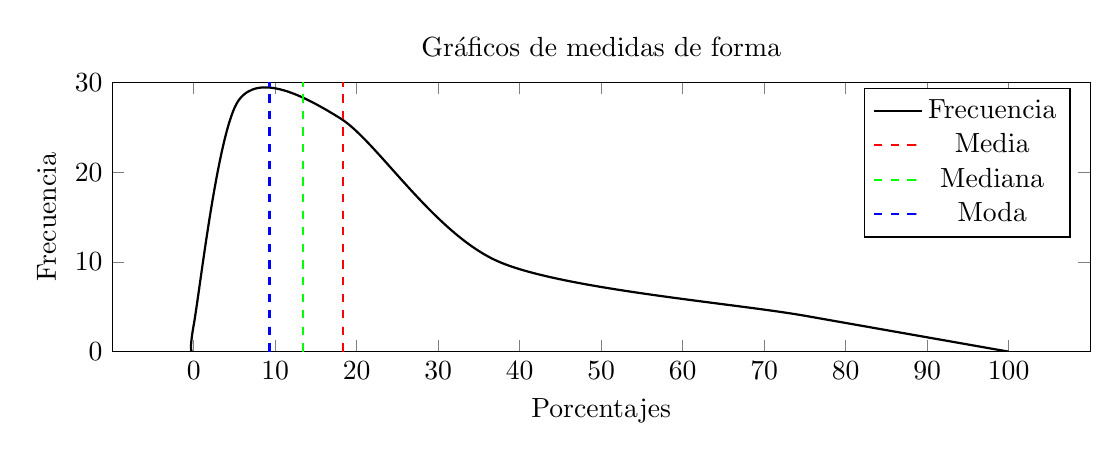
\begin{tikzpicture}
		\begin{axis}[
			width=14cm, height=5cm,
			xlabel={Porcentajes},
			ylabel={Frecuencia},
			xtick={0,10,20,30,40,50,60,70,80,90,100},
			ymin=0, ymax=30,
			grid=none,
			smooth,
			tension=0.5,
			title={Gráficos de medidas de forma}
			]
			\addplot[
			color=black,
			thick
			]coordinates{
				(0,0)
				(0,3)
				(5.5,28)
				(18,26)
				(37.5,10)
				(75,4)
				(100,0)
			};
			
			\addplot[
			color=red,
			thick,
			dashed
			]coordinates{(18.3,0)(18.3,30)};
			
			\addplot[
			color=green,
			thick,
			dashed
			]coordinates{(13.4,0)(13.4,30)};
			
			\addplot[
			color=blue,
			thick,
			dashed
			]coordinates{(9.3,0)(9.3,30)};
			\legend{Frecuencia, Media, Mediana, Moda}
		\end{axis}
	\end{tikzpicture}
	\vspace{-0.4cm}
	\caption{Distribución positiva y leptocúrtica}
\end{figure}
\vspace{-0.8cm}
\textbf{Interpretación de la información:} Los resultados indican que la mayoría de los participantes percibe un bajo nivel de automatización de tareas gracias a la IA, con un 36.36\% estimando entre un 1\% y un 10\% de automatización, y un 41.56\% entre un 11\% y un 25\%. La media de 18.25\% y la mediana de 14.28\% reflejan esta tendencia, con una ligera asimetría positiva que indica una mayor concentración de respuestas en los valores bajos. La curtosis leptocúrtica (0.43) sugiere que las respuestas se agrupan cerca de la media, lo que refuerza la idea de que la implementación de la IA es aún limitada y se aplica en tareas específicas.
